\documentclass[12pt]{beamer}

\hypersetup{colorlinks=true,linkcolor = blue}
\usetheme{Warsaw}

\usepackage[utf8]{inputenc}
\usepackage[russian,english]{babel}
\usepackage[T2A]{fontenc}

\usepackage{hyperref}
\usepackage[final]{listings}
\usepackage{breakurl}
\usepackage{cite}
\usepackage{perpage}

\def\Url\Breaks{\do\/\do-}

\lstset{
  frame=single,
  breaklines=true,
  basicstyle=\small,
  postbreak=\raisebox{0ex}{\ensuremath{\hookrightarrow\space}},
  numbers=left
}

\MakePerPage{footnote}

\title{Operating Systems}
\subtitle{Physical and Virtual Memory}
\author{Me}
\date{\today}

\begin{document}

  \begin{frame}
    \titlepage
  \end{frame}

  \begin{frame}
\frametitle{План}

\begin{enumerate}
  \item Расположение физической памяти.
  \item Понятие процесса и виртуальная память.
  \item Сегментация памяти как способ защиты.
  \item Paging и Page Fault.
  \item Аллокация непоследовательных страниц.
\end{enumerate}
\end{frame}

  \begin{frame}
\frametitle{Как выглядит физическая память?}

\only<1>{
\begin{figure}
  \centering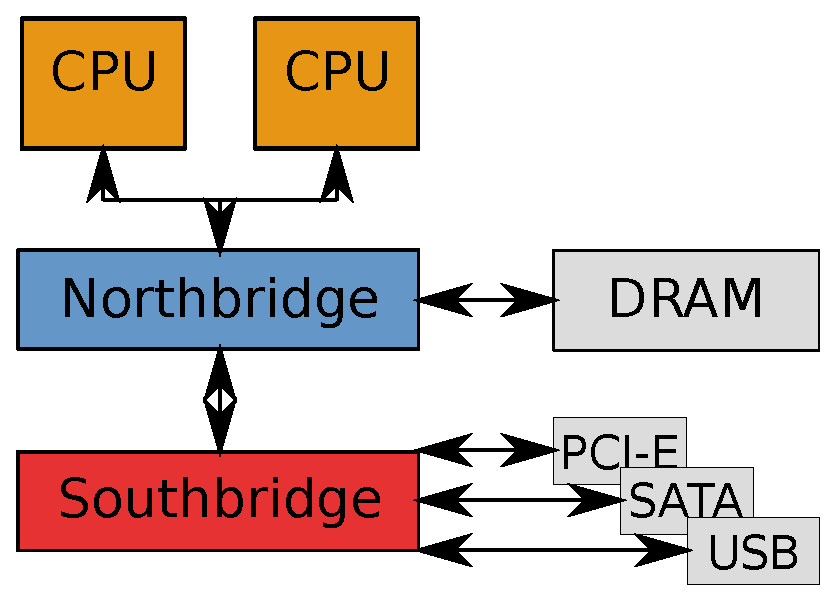
\includegraphics[width=.8\linewidth]{arch-uma}
  \caption{Classical UMA Architecture}
\end{figure}}
\only<2>{
\begin{figure}
  \centering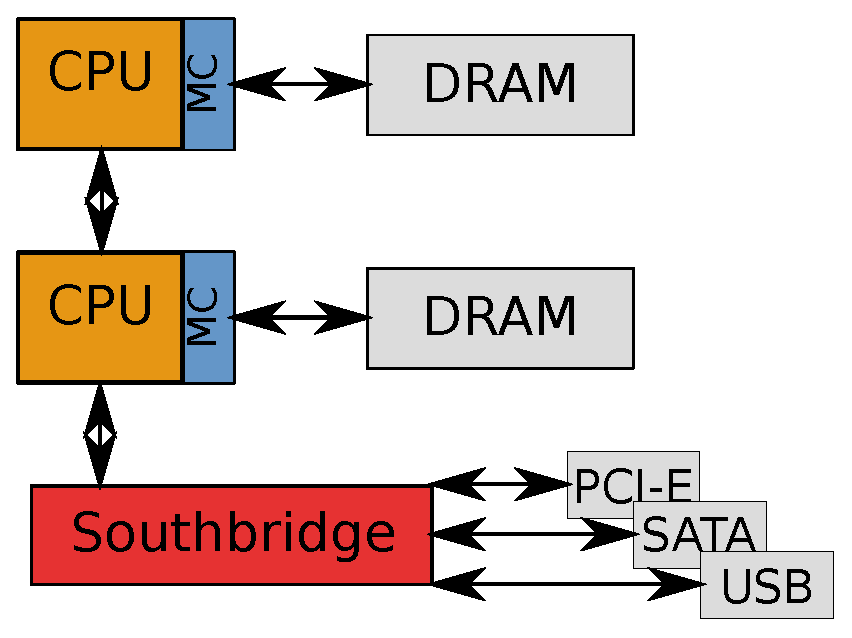
\includegraphics[width=.8\linewidth]{arch-numa}
  \caption{NUMA Architecture}
\end{figure}}

\end{frame}

\begin{frame}
\frametitle{Как выглядит физическая память?}

\onslide<1->{
Память не однородна:

\begin{itemize}
  \item адреса могут вообще быть не доступны - память не отображена никуда;
  \item адреса могут быть отображены на устройства - особые правила доступа/кеширования;
  \item разные адреса могут иметь разное время доступа с разных CPU (NUMA);
\end{itemize}}

\onslide<2->{Нужна карта памяти!}

\end{frame}

\begin{frame}
\frametitle{Где взять карту памяти?}

\begin{itemize}
  \item<1-> из документации чипсета
  \item<2-> из device tree
    \begin{itemize}
      \item кто-то все равно должен взять документацию чипсета и описать память в нужном формате и передать загрузчику
    \end{itemize}
  \item<3-> BIOS/UEFI или их аналог
    \begin{itemize}
      \item BIOS int \$0x15, функции 0xe820 или 0xe801
      \item UEFI GetMemoryMap
    \end{itemize}
  \item<4-> спросить у загрузчика (где ее берет загрузчик - не наше дело)
\end{itemize}
\end{frame}

\begin{frame}
\frametitle{Типичная карта памяти}

Такие регионы памяти, например, может сообщать QEMU через multiboot загрузчик:

\begin{itemize}
  \item \texttt{0x00000000-0x0009fbff, Available}
  \item \texttt{0x0009fc00-0x0009ffff, Reserved}
  \item \texttt{0x000f0000-0x000fffff, Reserved}
  \item \texttt{0x00100000-0x07ffdfff, Available}
  \item \texttt{0x07ffe000-0x07ffffff, Reserved}
  \item \texttt{0xfffc0000-0xffffffff, Reserved}
\end{itemize}

\end{frame}

  \begin{frame}
\frametitle{Понятие процесса}

Процесс - контейнер ресурсов ОС:
\begin{itemize}
  \item<2-> ресурсы в ОС привязаны к процессам
    \begin{itemize}
      \item память (свое адресное пространство у процессов)
      \item файловые дескрипторы
      \item другие ресурсы (сокеты, различные IPC и тд)
    \end{itemize}
  \item<3-> процессы изолированы друг от друга
    \begin{itemize}
      \item на сколько это позволяет аппаратное обеспечение (далее просто HW)
      \item некоторые процессы могут разделять общие ресурсы намеренно
    \end{itemize}
\end{itemize}

\end{frame}

\begin{frame}
\frametitle{Адресное пространство процесса}

Адресное пространство процесса (виртуальное адресное пространство, VA) - это набор адресов доступных процессу для работы (мы называем эти адреса виртуальными):

\begin{itemize}
  \item<2-> VA отображается на физическую память (далее PA)
    \begin{itemize}
      \item paging - произвольное отображение
      \item "один к одному", если HW не поддерживает трансляцию
    \end{itemize}
  \item<3-> VA может быть аппаратно защищено
    \begin{itemize}
      \item сегментирование - попытка обращения в чужой сегмент приводит к ошибке
      \item paging устраняет саму возможность обратиться к чужой памяти
    \end{itemize}
  \item<4-> VA может быть неоднородным - в нем могут быть дыры
\end{itemize}
\end{frame}

\begin{frame}
\frametitle{Адресное пространство процесса}

VA процесса - это ресурс, который нужно аллоцировать и освобождать:
\begin{itemize}
  \item<2-> ОС необходимо делить память между несколькими процессами - не нужно
выдавать процессу сразу много памяти, которая скорее всего не будет
использрована;
  \item<3-> разные части VA используются под разные нужды:
    \begin{itemize}
      \item они находятся в разных регионах VA (стек растет вниз, его логично положить наверх)
      \item могут иметь разные права/привелегии доступа (например, делать стек исполняемым - плохая затея с точки зрения безопасности)
    \end{itemize}
\end{itemize}
\end{frame}

\begin{frame}
\frametitle{Сегментация на примере x86}

Вся память разбивается на сегменты:
\begin{itemize}
  \item уровень привелегий доступа назначается каждому сегменту отдельно
  \item сегменты могут перекрываться, т. е. два сегмента с разными привелегиями могут описывать одну и ту же физическую память
\end{itemize}

\end{frame}

\begin{frame}
\frametitle{Сегментация на примере x86}

\begin{figure}
\centering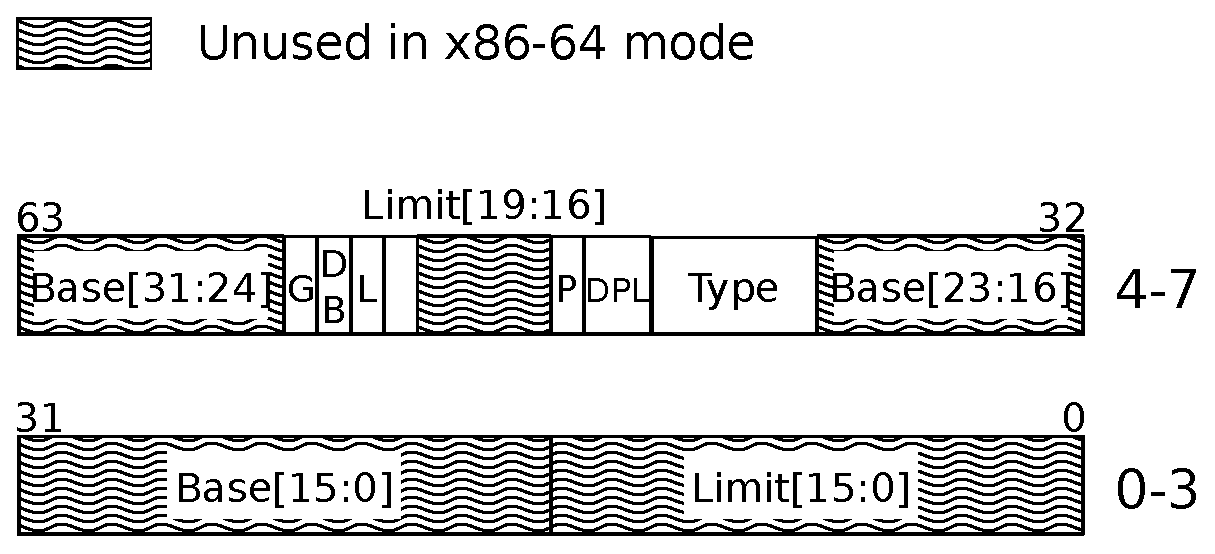
\includegraphics[width=.9\linewidth]{arch-segd}
\caption{x86 segment data/code descriptor format}
\end{figure}

\end{frame}

\begin{frame}
\frametitle{Сегментация на примере x86}

Дескрипторы сегментов хранятся в таблицах GDT и LDT:
\begin{itemize}
  \item GDT предполагается общей для всех процессов (не обязательно)
  \item LDT своя для каждого процесса (не обязательно)
  \item при обращении к памяти таблица и номер дескриптора в ней определяются используя селектор сегмента (16-битное значение в CS, SS, DS, ES, FS или GS)
\end{itemize}
\end{frame}

\begin{frame}
\frametitle{Сегментация на примере x86}

\begin{figure}
  \centering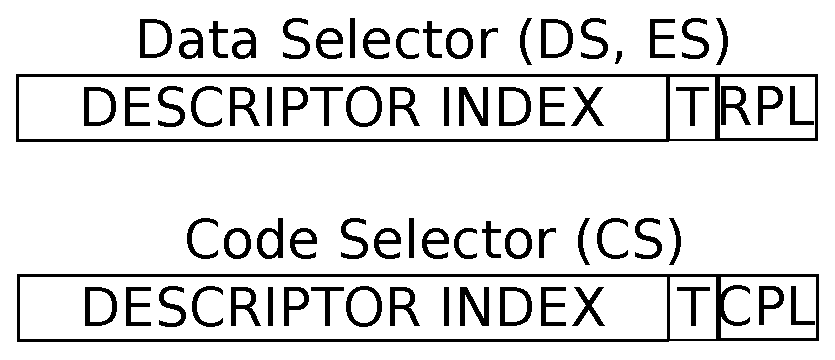
\includegraphics[width=.9\linewidth]{arch-segs}
  \caption{Code and Data Segment Selectors}
\end{figure}

\end{frame}

\begin{frame}
\frametitle{Сегментация на примере x86}

Проверка привелегий:
\begin{itemize}
  \item при записи селектора в сегментный регистр CPL (из CS) и RPL (то что мы записываем) должны быть меньше или равны DPL (в дескрипторе сегмента, на который мы ссылаемся);
  \item для селектора стека (SS) используются особые правила - RPL и DPL должны быть равны CPL.
\end{itemize}
\end{frame}


%  \begin{frame}
%    \bibliography{lec3}{}
%    \bibliographystyle{apalike}
%  \end{frame}

\end{document}
